\documentclass{article}
\usepackage[utf8]{inputenc}
\RequirePackage[numbers]{natbib}
\usepackage[intoc,french]{nomencl}
\makenomenclature
\renewcommand{\nomname}{Notations}
\usepackage{etoolbox}
\usepackage{subcaption}
\usepackage{graphicx}
\usepackage{enumitem} 
\usepackage{fancyhdr}
\usepackage[utf8]{inputenc}
\usepackage{amsmath, amssymb, amsthm}
\usepackage[top=3cm, bottom=3cm, left=2cm, right=2cm]{geometry}

\title{Spécification d'histogrammes dans le cas de zones constantes}
\author{Pierre Dubreuil, Thomas Eboli}

\begin{document}
\maketitle

\begin{abstract}
Dans ce rapport, nous allons présenter nos résultats au sujet d'application de la spécification d'histogrammes au traitement des images. Nous nous sommes appuyé sur le code fourni par madame Nikolova ainsi que sur le papier de base. La première étape du travail, en amont de tout bout de code a été de comprendre les enjeux soulevés par le papier et d'appréhender la puissance du speed-up de la phase "d'ordering" dans le problème de la spécification d'histogrammes. L'un des principaux problèmes que nous avons cherché à résoudre est l'a présence de "large pixels" dans les images obtenues après spécification. Notre méthode de résolution repose sur des considérations probabilistes d'un histogramme comme la distribution de probabilité d'une variable aléatoire $X$ qui est ici l'image.
\end{abstract}

\paragraph*{}
Ce document est organisé comme suit: la partie 1 est dédiée à présenter le problème de "large pixels" et d'en comprendre la source. La partie 2 présente notre première approche pour résoudre le problème ainsi que que les résultats obtenus. La partie 3 s'intéressera à des méthodes de dithering plus récentes et plus efficaces pour résoudre des problèmes de quantifications de palette de couleur comme l'algorithme d'Atkinson. 

\section*{Présentation du problème de "large pixels"}
\paragraph*{}
Lors de l'application de l'algorithme donné, on s'aperçoit que les images font apparaître des détails que l'on ne veut pas. La figure \ref{fig:p1_brasil} illustre à merveille ce phénomène qui découle de la mauvaise quantification de la palette de couleurs dans la nouvelle configurations de bits de couleurs. En effet les figures \ref{fig:im_x} et \ref{fig:im_xx} montrent que la spécification d'histogramme, lorsque l'histogramme cible est très différent de l'original, déplace des pixels d'un certain niveau de couleur vers des régions où il n'y avait pas de pixels pour colorer avec cette teinte. Le résultat est visible sur ces figures; le contraste est beaucoup plus riche et la photographie du port de Malte est moins terne mais on fait apparaître dans le ciel des blocs de pixels blancs. Ces pixels sont le résultat d'une volonté de rendre plus contrastée cette zone de l'image mais l'image originale ne possédant qu'une zone quasi constante de couleurs, la nouvelle allocation arrive à rendre le dégradé souhaité que par de gros tas de pixels, les "large pixels". Il faut donc arriver à trouver une technique permettant de gommer ces détails liés à des zones planes dans les images de départ.

\begin{figure}[!hbt]
\centering
\begin{minipage}{0.5\textwidth}
\centering
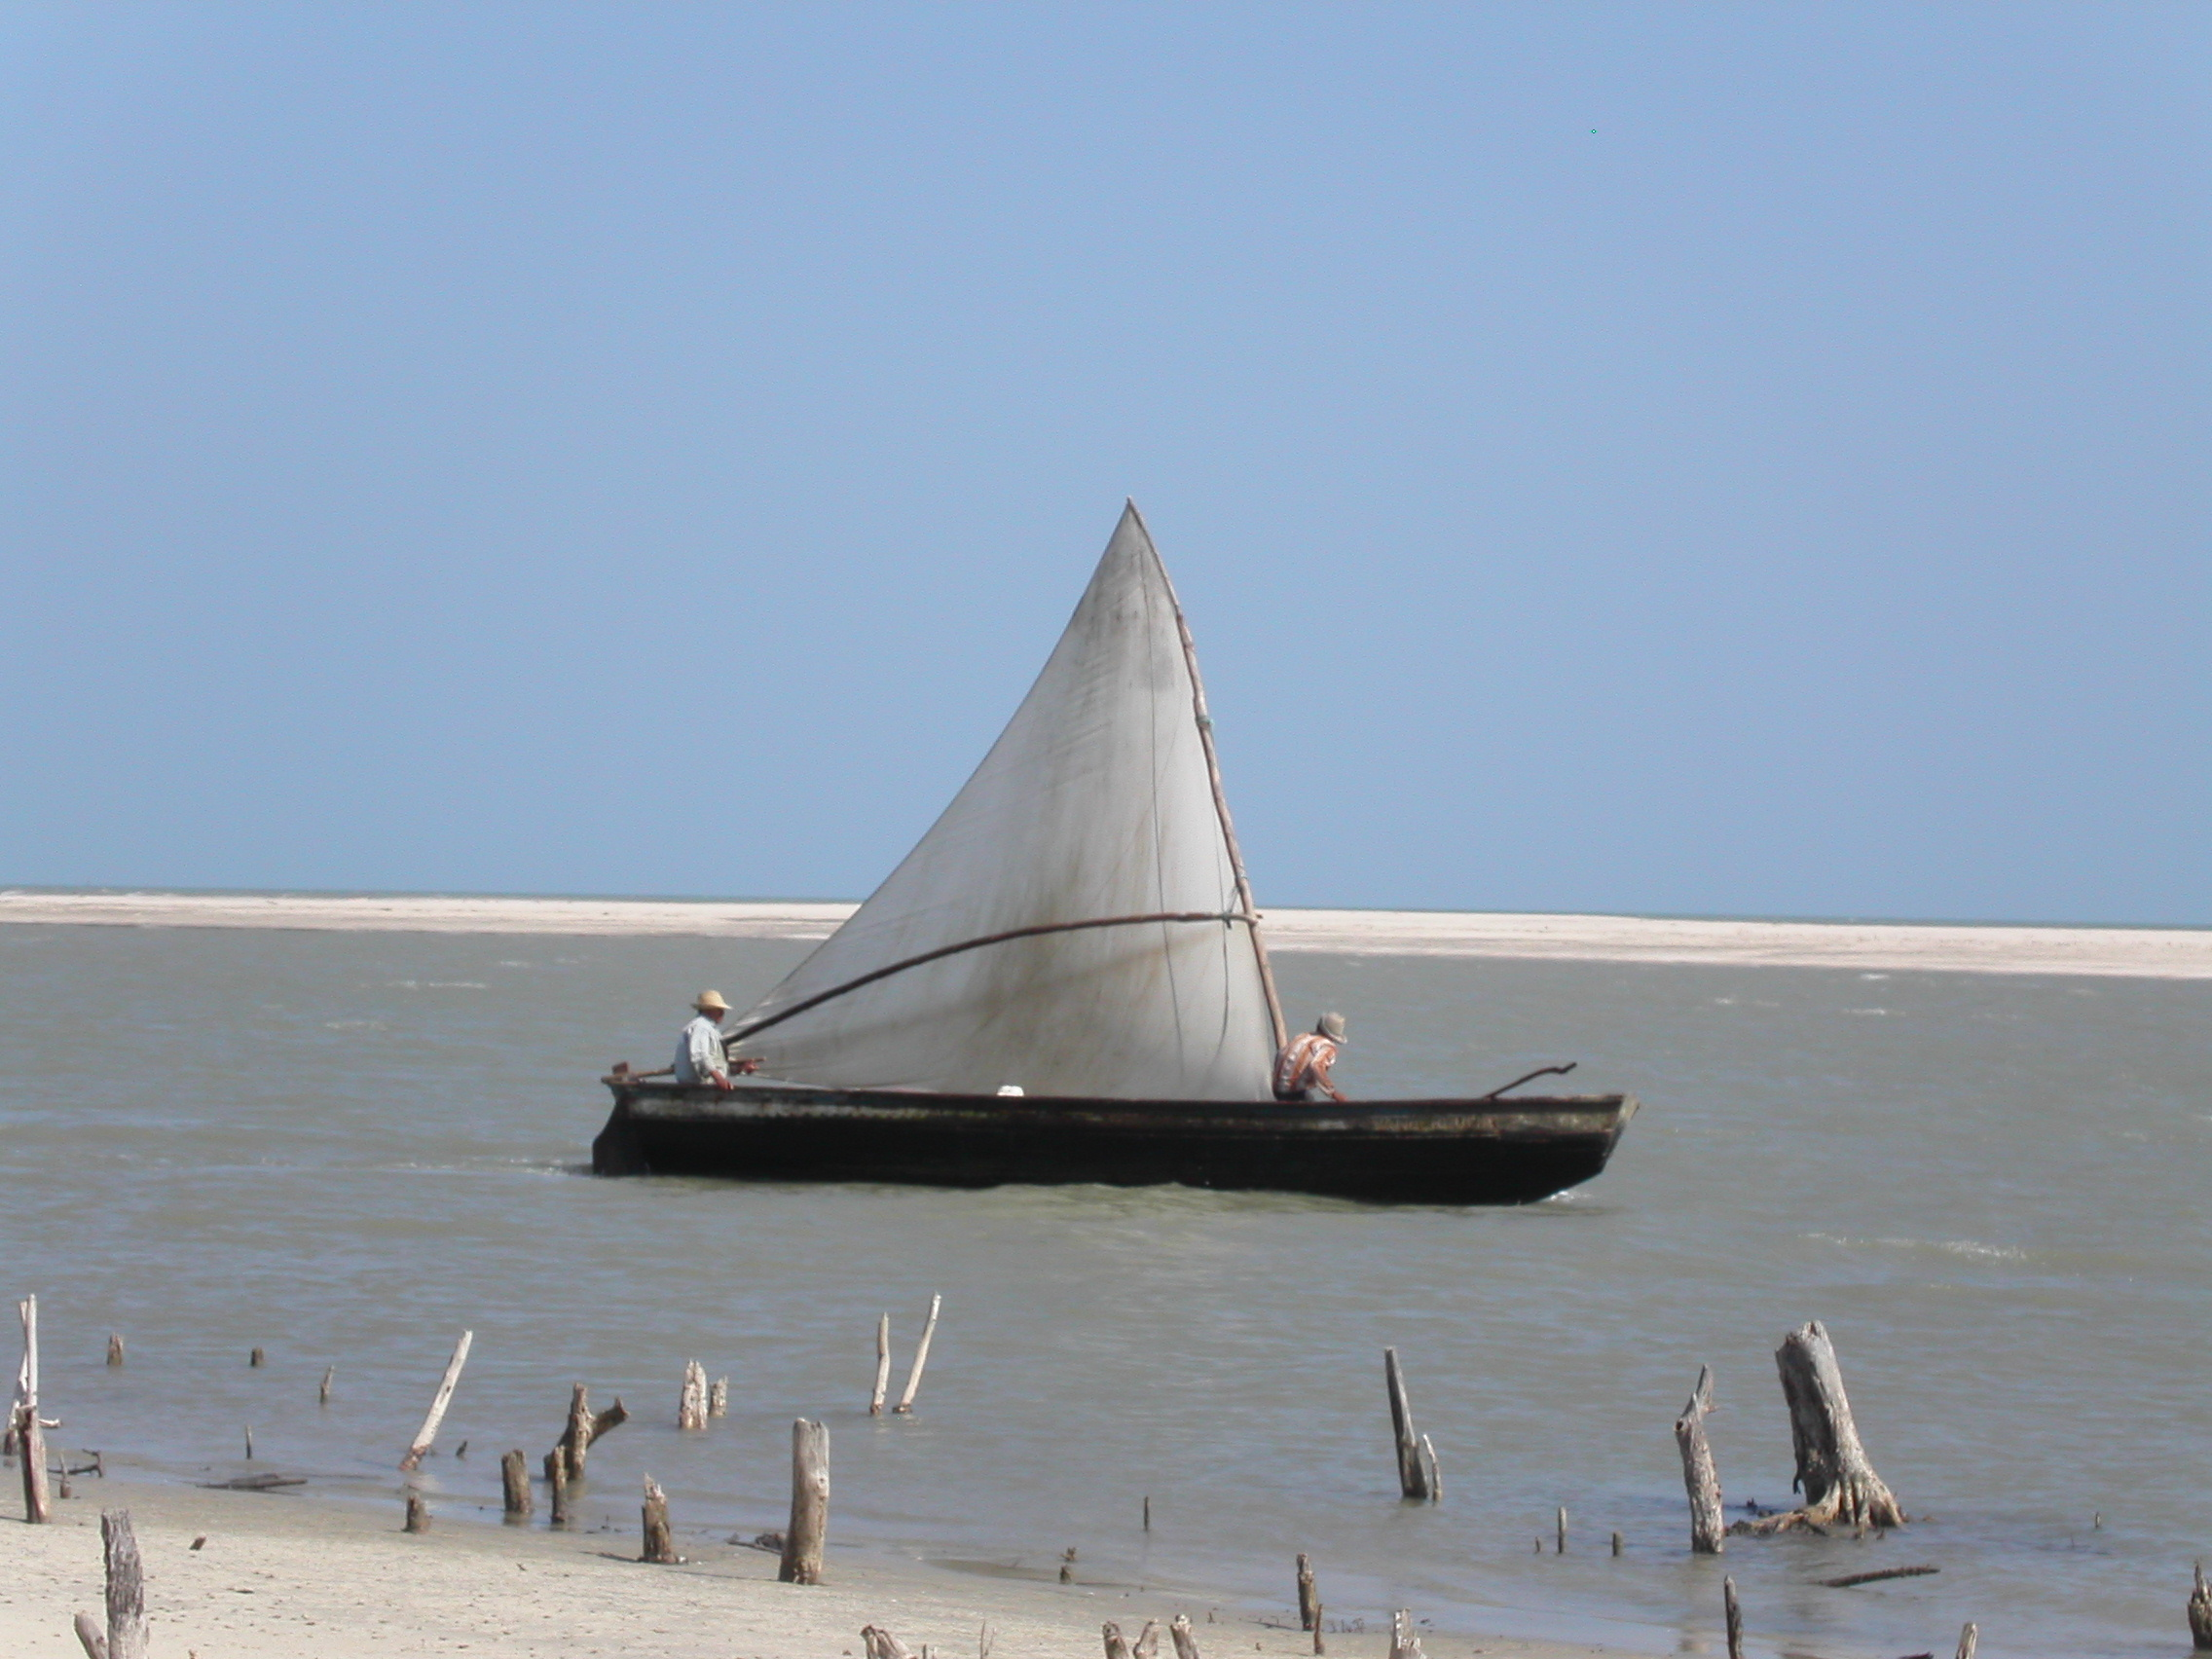
\includegraphics[width=0.75\textwidth]{../pictures/brasil.jpg}
\end{minipage}%
\begin{minipage}{0.5\textwidth}
\centering
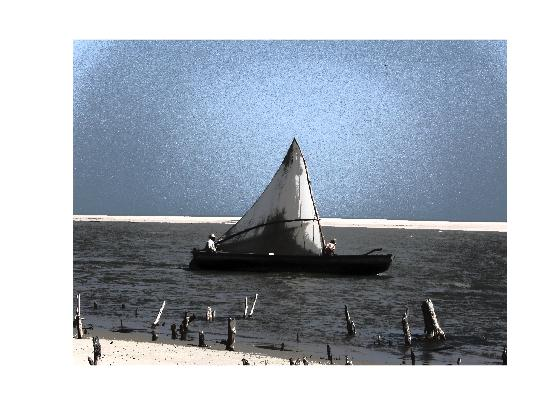
\includegraphics[width=0.98\textwidth]{images/p1_brasil.jpg}
\end{minipage}
\caption{\textit{Illustration de l'apparition de pixels nuisibles dûs à la ré-allocations de bits dans l'histogramme produisant une mauvaise quantification des couleurs.}}
\label{fig:p1_brasil}
\end{figure}

\begin{figure}[!htb]
\centering
\begin{minipage}{0.5\linewidth}
\centering
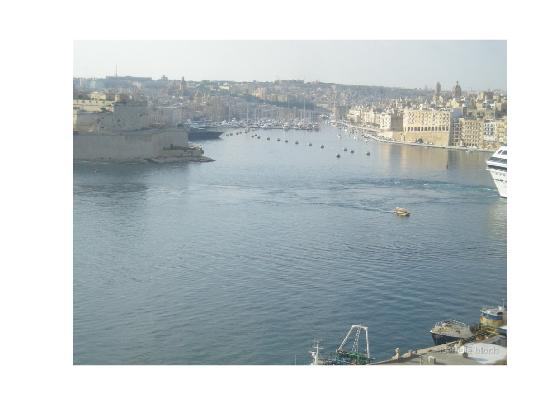
\includegraphics[width=0.98\linewidth]{images/im_x.jpg}
\end{minipage}%
\begin{minipage}{0.5\linewidth}
\centering
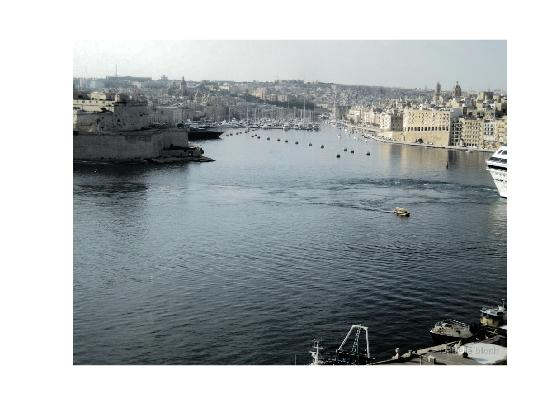
\includegraphics[width=0.98\linewidth]{images/im_xx.jpg}
\end{minipage}
\caption{\textit{Image de départ et son équivalent après spécification. On remarque qu'en haut à gauche, il y a des pixels apparents dans le ciel dûs à une mauvaise allocation des couleurs après spécification d'histogramme.}}
\label{fig:im_x}
\end{figure}

\begin{figure}[!hbt]
\centering
\begin{minipage}{0.33\textwidth}
\centering
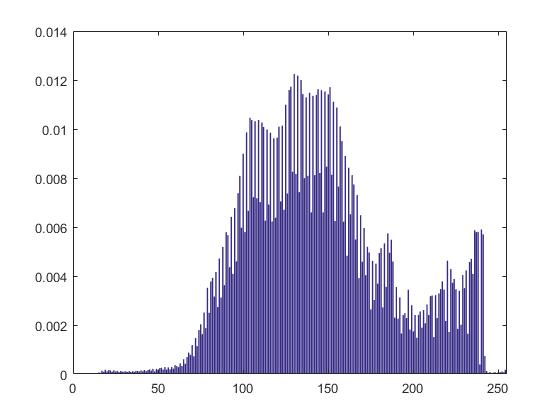
\includegraphics[width=0.98\textwidth]{images/hist_x.jpg}
\end{minipage}%
\begin{minipage}{0.33\textwidth}
\centering
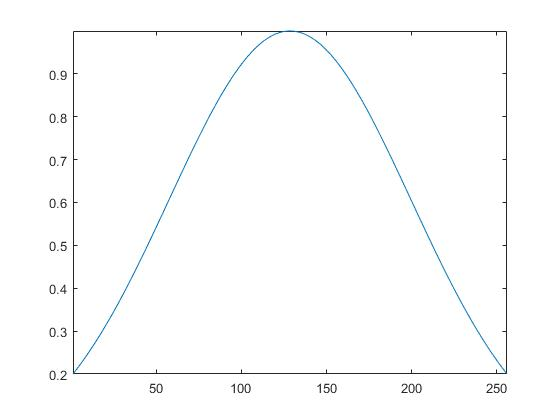
\includegraphics[width=0.98\textwidth]{images/p1_hist_cible_malte.jpg}
\end{minipage}%
\begin{minipage}{0.33\textwidth}
\centering
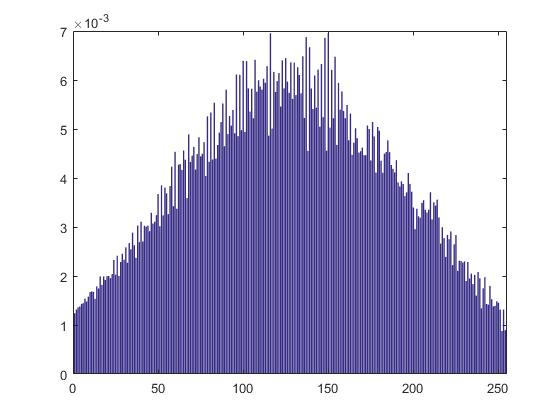
\includegraphics[width=0.89\textwidth]{images/hist_xx.jpg}
\end{minipage}
\caption{\textit{Gauche: histogramme de départ, Milieu: forme de l'histogramme cible, Droite: histogramme obtenu après application de la spécification par la routine order}}
\label{fig:im_xx}
\end{figure}

\section*{Divers pistes}
\paragraph*{}
Dans cette section, nous souhaitons faire part des différentes approches que nous avons entrepris pour résoudre le problème de "large pixel". 

\subsection*{Approche par tilling}
Une première idée a été de vouloir traiter des bouts d'images indépendamment les uns des autres car le problème est souvent localisé dans certaines zones de l'image. Les approches par tilling et pyramides multi-échelles étant monnaie courante en traitement des image, nous avons voulu l'essayer dans notre problème. Malheureusement, qui dit tilling dit traitement séparé des informations ce qui ne nous arrange pas car nous voulons dispatcher l'ensemble des pixels de l'image et les réorganiser. Le résultat obtenu (sans utiliser d'algorithme type Midway qui aurait permis d'unifier les couleurs des différentes imagettes) n'est pas convaincant du tout car des zones claires et foncées apparaissent là où on le veut pas comme on peut le voir dans la figure \ref{fig:tilling} où les jonctions de chacune des imagettes pose problème. Cette figure a été obtenue avec une approche de type pyramide où chaque quart est la moyenne entre le quart de l'image de niveau 0 et l'imagette traitée à part au niveau 1 avec son propre histogramme (cf code dans le dossier "tilling").

\begin{figure}
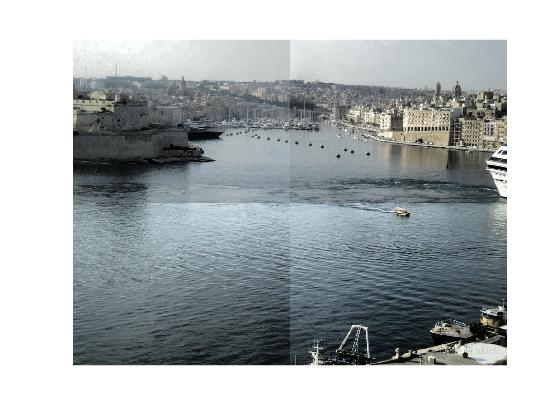
\includegraphics[scale=0.75]{images/p2_tilling.jpg}
\caption{\textit{Sans même se donner la peine de traiter l'image par un algorithme type midway pour unifier les couleurs, on aperçoit dans l'image en haut à droite que le ciel est un dégradé qui ne prend pas en compte le ciel de l'imagette en haut à gauche. Pire encore, le phénomène de "large pixels" est encore plus accentué car on a encore moins de bits à allouer aux zones claires ! Même constat pour chacune des jonctions.}}
\label{fig:tilling}
\end{figure}

\section*{Résolution par ajout de bruit}
\subsection*{Approche probabiliste}
\paragraph*{}
La partie précédente met en évidence que le transport d'un histogramme d'une image réelle vers un histogramme cible ne peut se faire complètement ce qui laisse apparaître des défauts dans l'image générée à partir du nouvel histogramme obtenu.
\subparagraph*{}
Comme annoncé dans l'introduction, nous sommes partis du constat qu'une image est la réalisation d'une variable aléatoire $X$ vivant dans un espace de très grande dimension (de l'ordre du million en pratique) et que son ou ses histogrammes, selon que X est une image couleur ou en niveau de gris, représentent les distributions de probabilités de chacun des canaux. Dans ce contexte, on peut utiliser un résultat classique de probabilités:
\paragraph*{Théorème 1:} Soient $x$ et $y$ les réalisations de deux variables aléatoires $X$ et $Y$ de densités respectives $f_x$ et $f_y$. Alors $x+y$ est aussi une variable aléatoire suivant la loi $X+Y$ et de densité $f_x * f_y$.
\subparagraph{} Toutes les considérations suivantes seront prises sur des images en niveaux de gris. Pour appliquer les résultats à des images couleurs, il suffit d'appliquer les calculs à chacun des canaux. On considérant maintenant que $x$ est notre image et en notant $b$ le bruit (gaussien, uniforme, peu importe), on obtient que l'image $x_b = x+b$ possède un histogramme qui s'écrit $h_x * h_b$. On peut donc maintenant jouer sur le type de bruit et son écart-type $\sigma$ pour modifier l'allure de l'histogramme  de $x$ et donc modifier en aval le contraste de manière plus fine.
\subparagraph*{} Théoriquement, on arrive alors a moyenner l'histogramme de x. On définit la valeur d'un bin $h_{x_b}(i)$ pour $i \in {0,...,255}$ comme une fonction de de $h_x(i)$ mais aussi de ses voisins. On force donc l'histogramme avoir des valeurs plus faibles aux endroits où il n'y avait pas de pixels au départ ce qui réduit l'apparition de motifs invisible au début et qui deviennent visibles par la suite. Le choix du type de bruit à appliquer définit donc le type de moyenne qu'on utilise. Par exemple un bruit uniforme appliquera une moyenne classique aux bins de l'histogramme de $x$.

\subsection*{Résultats}

\section*{Méthodes de dithering plus récentes}
\paragraph*{}
L'idée d'ajouter du bruit à l'image pour casser ces zones constantes n'est pas nouvelle et date du milieu des années 50. Entre temps, le domaine de la quantification des palettes de couleurs a connu un grand intérêt avec l'arrivée des écrans couleurs. La trame de Bayer est l'un des exemples les plus connus, permettant de coloriser par des hachures des images. Globalement cette technique fonctionne bien mais fait apparaître des artefacts dans les zones hautes-fréquences. Notre problème étant celui de traiter de coloriser des zones de teinte constante qui deviennent à teinte variable après application de l'algorithme. La littérature à ce sujet est assez riche et plusieurs algorithmes sont disponibles comme celui de Floyd et Steinberg de 1975. Nous avons choisi l'algorithme d'Atkinson datant des années 80 qui repose sur la technique de Floyd et Steinberg mais est plus rapide et donne de meilleurs résultats.
\subparagraph*{}
Le principe de ces algorithmes est assez simple. Pour chaque pixel codé, on attribut une valeur $q_i$ appartenant aux valeurs de quantifications possibles $q_j$, $\forall j \in {1,..., L}$ puis on garde en mémoire l'erreur entre cette valeur quantifiée $q_i$ et la véritable valeur de ce pixel. On la propage aux pixels voisins et on quantifie la valeur voisine en ajoutant l'erreur de quantification du premier pixel ce qui permet de créer des structures en damier ou des sortes de patchworks plus ou moins denses de pixels noirs et blancs pour donner l'impressions de plusieurs teintes de gris alors qu'on a que deux couleurs. Dans le cas des images couleurs, le procédé est appliqué à chacun des canaux de couleurs.
\subparagraph*{}
Avec cette procédure simple mais astucieuse, on arrive à gommer beaucoup des erreurs de quantifications. L'idée du procédé n'est pas étrangère à notre première approche du problème car même si nous avons pensé en terme d'histogramme au début, ajouter du bruit revient à casser la redondance des zones constantes et donc à donner un aspect plus contraster et moins bloc de couleurs dans les zones unis, les zones hautes-fréquences ne faisant pas ressortir le grain du bruit.

\subsection*{Résultats}

\end{document}